%http://cms-results.web.cern.ch/cms-results/public-results/preliminary-results/SUS-16-024/index.html

%% CVSId: $Id: Example.tex,v 1.1.1.1 2000/11/28 11:15:12 exupery Exp $
\documentclass[%
xcolor=dvipsnames,table%,pdftex%,
%pdf,
%nocolorBG,
%colorBG,
%slideColor,
%slideBW,
%draft,
%frames
%azure
%contemporain
%nuancegris
%troispoints
%lignesbleues
%darkblue
%alienglow
%autumn
%12pt
]{beamer}
%%%%%%%%%%%%%%%%%%%%%%%%%%%%%
%\mode<presentation>
%{
  %\usetheme{Madrid}
 \usetheme[progressbar=frametitle]{m}% \usetheme{Boadilla}
  % or ...
%%%%%%%%%%%%%%%%%%%%%%%%%%%%%%%%%%%%%
%para revelar texto a aparecer en overlays
  %\setbeamercovered{transparent} 
  %\setbeamercovered{invisible}
%%%%%%%%%%%%%%%%%%%%%%%%%%%%%%%%%%%%%
  % \setbeamertemplate{blocks}[rounded][shadow=true]
  % \setbeamertemplate{navigation symbols}{}

  % \setbeamertemplate{footline}{%\hspace*{.5cm}
  %   \scriptsize{\phantom{Gg}%\insertauthor 
  %     \hspace*{50pt} 
  %     \hfill \insertframenumber
  %     \hspace*{.5cm}}}

  % % or whatever (possibly just delete it)
  % %\useoutertheme{shadow} 
  % \setbeamercolor{postit}{fg=black,bg=yellow}
  % \setbeamercolor{white}{fg=black,bg=white}
  % \setbeamercolor{cite}{fg=black,bg=yellow}
%}


\usepackage[absolute,overlay]{textpos}
\usepackage{booktabs}
\usepackage[scale=2]{ccicons}

%\usepackage{pgfplots}
%\usepgfplotslibrary{dateplot}

%%%%%%%%%%%%%%%%%%%%%%%%%%%%%%
%Force pdflatex processing even with "$ latex" (required by arXiv)
%\pdfoutput=1
\graphicspath{{figures/}}
%\usepackage[T1]{fontenc}
%\usepackage[utf8]{inputenc}
%\usepackage[spanish]{babel}
%\spanishdecimal{.}
%\usepackage{marvosym}
%\usepackage{beamerprosper}
\usepackage{amsmath,amssymb}
\usepackage{overpic}
\usepackage{graphicx}
\usepackage{mycolors}
%\usepackage{xmpmulti}
\usepackage{multimedia}
\usepackage{pgf}
\usepackage{cancel}
\usepackage{wasysym}
%\usepackage{helvet}
\usepackage{comment}
\usepackage{array}   % for \newcolumntype macro
\newcolumntype{L}{>{$}l<{$}} % math-mode version of "l" column type
\includecomment{comentar}
\specialcomment{comentar}
{\begingroup}{\medskip\endgroup}
\excludecomment{comentar}

\includecomment{comentario}
\specialcomment{comentario}
{\begingroup}{\endgroup}
\excludecomment{comentario}

\includecomment{details}
\specialcomment{details}
{\begingroup}{\endgroup}
\excludecomment{details}

%\usepackage[texcoord,grid,gridunit=mm,gridcolor=red!10,subgridcolor=green!10]{eso-pic}


\newcommand{\widescreen}{
\setlength{\paperwidth}{171 mm}
\setlength{\paperheight}{96 mm}
\setlength{\textwidth}{161 mm}
\setlength{\textheight}{86 mm}
}

%\widescreen


\title{Phenomenology of scotogenic models}
\subtitle{LHC signals  }


%\subtitle
%{Reconstruction of the neutrino mass matrix} % (optional)

\author{Diego Restrepo}
% - Use the \inst{?} command only if the authors have different
%   affiliation.
\institute{
  \begin{columns}
    \begin{column}{0.5\textwidth}
Instituto de F\'\i sica\\
Universidad de Antioquia\\
Phenomenology Group\\
\url{http://gfif.udea.edu.co}      
    \end{column}
    \begin{column}{0.5\textwidth}
      \hfill SILAFAE-2016\\
      \hfill \includegraphics[scale=0.15]{volcano}\\
      \hfill \tiny{Volcán de Fuego (Caroline Kish)}
    \end{column}
  \end{columns}
\quad\\
\quad\\
{\tiny
\alert{\textbf{Focus on}} \\
arXiv: arXiv:1308.3655 (JHEP),
arXiv:1504.07892 (PRD),
arXiv:1509.06313 (PRD),
arXiv:1511.01873 (JHEP),
arXiv:1605.01129 (PRD)\\
\alert{In collaboration with}\\
  G.~Palacio, F.~von~der~Pahlen, D.~Portillo, A.~Rivera, M.~Sánchez, O.~Zapata (UdeA)\\
  C. Arbeláez (USM), W.~Tangarife (Tel Aviv U.), C.~Yaguna  (Heidelberg, Max Planck Inst.).}\\
%\centering
}
% - Use the \inst command only if there are several affiliations.
% - Keep it simple, no one is interested in your street address.

\date{\tiny November 15, 2016 } % (optional) \today
%{
\includegraphics[scale=0.3]{udea}}
\titlegraphic{\hfill
\includegraphics[height=1.5cm]{udea}}

%\subject{Talks}
% This is only inserted into the PDF information catalog. Can be left
% out. 



% If you have a file called "university-logo-filename.xxx", where xxx
% is a graphic format that can be processed by latex or pdflatex,
% resp., then you can add a logo as follows:

% \pgfdeclareimage[height=0.5cm]{university-logo}{university-logo-filename}
% \logo{\pgfuseimage{university-logo}}



% Delete this, if you do not want the table of contents to pop up at
% the beginning of each subsection:
%\AtBeginSubsection[]
%{
%  \begin{frame}<beamer>
%    \frametitle{Outline}
%    \tableofcontents[currentsection,currentsubsection]
%  \end{frame}
%}

\newcommand{\chml}[2]{$\underline{\text{#1\hspace{#2}}}$}
\begin{document}


%===============
\begin{comentar}
%===============  
%=============
\end{comentar}
%=============

\maketitle
 % \begin{frame}%[plain]
 %   \titlepage
 % \end{frame}
% }



% {
% \usebackgroundtemplate{\includegraphics[width=\paperwidth]{tocrs}}
\begin{frame}
  \frametitle{Table of Contents}
\small
%\vspace{-0.5cm}
  \setbeamertemplate{section in toc}[sections numbered]
  \tableofcontents[hideallsubsections]
\end{frame}


\section{General framework}

% * <restrepo@udea.edu.co> 2015-11-15T12:41:09.269Z:
%
% Rememeber the basic idea: combine nu and dark matter
%
% ^.

\begin{frame}
  \frametitle{$\nu$-DM models}
  \only<1->{\alert{small neutrino masses}}%
\only<1>{\phantom{ $\Leftarrow Z_2 \Rightarrow$ \alert{dark matter} }}%
\only<2>{ $\color{red}\Leftarrow Z_2 \Rightarrow$ \alert{dark matter} }
\only<1>{
  \begin{figure}
    \centering
    \includegraphics[scale=0.9]{nudm1}
  \end{figure}
}%
\only<2>{
  \begin{figure}
    \centering
    \includegraphics[scale=0.9]{nudm2}
  \end{figure}
}%
\only<1>{\phantom{35 non-equivalent dark matter models classified in}}%  
\only<2>{{35 non-equivalent dark matter models classified in}}
  
\only<1>{\phantom{D.R., C. Yaguna, O. Zapata,  arXiv:1308.3655 (JHEP)}}%
\only<2>{{D.R., C. Yaguna, O. Zapata,  arXiv:1308.3655 (JHEP)}}

\only<1>{\phantom{{\color{green}2. Neutrinos talk to a different Higgs boson}}}
\only<2>{{{\color{Green}2. Neutrinos talk to a different \textbf{Higgs boson}}}}
% %


\end{frame}
%%%%%
%%%%%%%%%%%
\begin{frame}
\frametitle{Weinberg operator at one-loop}
\begin{picture}(320,250)
\only<1->{\put(-20,140){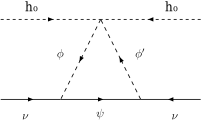
\includegraphics[scale=0.8]{T3}}}%
\only<1->{\put(160,140){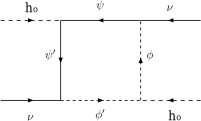
\includegraphics[scale=0.8]{T1-2}}}%
\only<1->{\put(-20,20){\includegraphics[scale=0.8]{T1-1}}}%
\only<1->{\put(160,20){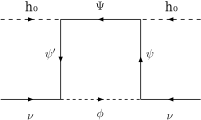
\includegraphics[scale=0.8]{T1-3}}}%
\only<2>{\put(-20,130){Wino-like scotogenic model}}
\only<2>{\put(150,13){\includegraphics[scale=0.1]{new}Higgsino-like scotogenic model}}
\only<2>{\put(150,130){\includegraphics[scale=0.1]{new}Higgsino-like Zee model}}
\only<2>{\put(55,118){$\Updownarrow$}}
\only<2>{\put(225,160){\tiny arXiv:1511.01873}}
\only<2>{\put(40,160){\tiny arXiv:1605.01129}}
\only<2>{\put(225,40){\tiny arXiv:1504.07892}}
\only<1->{\put(120,240){\color{red}($Z_2$-odd fields) }}
%\only<4->{\put(233,186){\fcolorbox{black}{blue}{\color{white}Zee model}}}%
\end{picture}
\end{frame}


\begin{frame}
   \frametitle{
\only<1>{Typical radiative neutrino mass diagram.}%
\only<2>{In term of general SU(2)${}_{L}$ multiplets,}%
\only<3>{may be also contain charged particles,}%
\only<4>{which may decay into the dark matter particle.}%
}
  \only<1>{\includegraphics[scale=1.5]{main_vertex1}}%
  \only<2>{\includegraphics[scale=1.5]{main_vertex2}}%
  \only<3>{\includegraphics[scale=1.5]{main_vertex3}}%
  \only<4>{\includegraphics[scale=1.5]{main_vertex4}}%
\end{frame}



\section{Proposal: $pp\to l^+l^-+{E_T^{\text{miss}}}$}
%%%%
\begin{frame}
  \frametitle{Dilepton plus transverse missing energy signal}
\vspace{-0.3cm}
  \begin{center}
    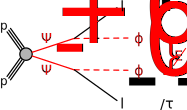
\includegraphics[scale=1]{fig_02ai}

\vspace{-0.2cm}

    $\operatorname{SU}(2)_L$ assignments:

\vspace{-0.8cm}
  \begin{align*}
    \color{red}
    \Psi=&\color{red}\boldsymbol{1},\boldsymbol{2} (\Psi),\boldsymbol{3} (\Sigma)\,,&\color{red}\Phi\color{red}=&\color{red}\boldsymbol{1},\boldsymbol{2}\,,\ \text{with}\ m_{\text{DM}}\sim m_{h}/2\,.
  \end{align*}
\vspace{-1.3cm}

\hrulefill

\vspace{-0.4cm}

Simplified SUSY models
  \end{center}
\vspace{-0.8cm}
  \begin{overpic}[scale=0.9%,grid
            ]{fig_02a}
    \put(26,48){$\color{red}\tilde{l}/$}    
    \put(26,23){$\color{red}\tilde{l}/$}    
    \put(73,70){$l/$}    
    \put(73,2){$l/$}    
    \put(-15,-10){Smaller cross sections.}    
  \end{overpic}\hfill
  \begin{overpic}[scale=0.9%,grid
            ]{fig_02b}
    \put(-70,-10){Intermediate states and smaller lepton $\cancel{\boldsymbol{p}_{\text{T}}}$}
    %\only<2>{\put(-180,180){\hspace{1cm}\color{blue} Benchmark point: 100 GeV \hspace{1cm}60 GeV }}    
  \end{overpic}
\end{frame}
% * <restrepo@udea.edu.co> 2015-11-15T12:45:09.589Z:
%
% Explanation of the framework
%
% ^.

\section{Specific examples}



\begin{frame}
  \frametitle{Specific examples}
  
  \begin{itemize}
    \item Wino-like scotogenic models
    \begin{itemize}
    \item \alert{Radiative type-III seesaw}: \tiny{1605.01129, 	
 F. von der Pahlen, G. Palacio, DR, O. Zapata}
    \end{itemize}
    \item Higgsino-like scotogenic models
      \begin{enumerate}
      \item SDFM with scalars: {\tiny 1504.07892, DR, \textit{et. al.}.}
      \item Inert Zee: {\tiny 1511.01873, R. Longas, D. Portillo, DR, O. Zapata.}
      \item \alert{Radiative type-II seesaw}: {\tiny 1511.06375, S. Fraser, C. Kownacki, E. Ma, O. Popov}\\
       \hspace{4.2cm}     {\tiny 1609.01018,   S. Guo, Z. Han, Y, Liao }
      \end{enumerate}
    \item Bino-like scotogenic models
      \begin{itemize}
      \item In progress ...
      \end{itemize}
  \end{itemize}


\end{frame}

\begin{frame}
  \frametitle{Wino-like {\tiny scotogenic model} \hspace{3.5cm} Higgsino-like  {\tiny \only<1>{inert Zee}\only<2>{scotogenic} model}}

\vspace{0.2cm}

\begin{columns}
  \begin{column}{0.5\textwidth}
\vspace{-1.2cm}

\only<1>{\includegraphics[scale=0.7]{rs_iii}}
\only<2->{\includegraphics[scale=0.7]{T1-1-a}}

\rowcolors{1}{RoyalBlue!20}{RoyalBlue!5}
\begin{tabular}{|c||c|c|c|c|c|}
\hline 
&  $SU(2)_{L}$ & $  U(1)_{Y}$   & $Z_2$ & $S$
\\ \hline \hline 
 $H$  & $2$&$ 1$ & $+$ & $0$ \\
\hline
 $\color{red}\Phi\phantom{_{\rm SM}}$ & $2$&$ 1$  & $-$ & $0$ \\
\hline
 ${L_\alpha}$  & $2$&$-1\phantom{-} $ & $+$ & $1/2$ \\
\hline 
 $\color{red}{\Sigma}_{k}$ & $3$&$ 0$  & $-$ & $1/2$ \\ 
\hline
\end{tabular} 
  \end{column}
  \begin{column}{0.5\textwidth}

\vspace{-0.2cm}

\only<1>{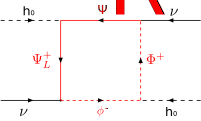
\includegraphics[scale=0.7]{T1-2-a}}
\only<2->{
\includegraphics[scale=0.7]{T1-3-a} }


\rowcolors{1}{RoyalBlue!20}{RoyalBlue!5}
\begin{tabular}{|c||c|c|c|c|c|}
\hline 
&  $SU(2)_{L}$ & $  U(1)_{Y}$   & $Z_2$ & $S$
\\ \hline \hline 
 $\color{red}\phi^{-}$ & $1$&$ -2$  & $-$ & $0$ \\ \hline
$\color{red}\Phi$ &2 & $-$& 0&-\\
\hline
\only<1-2>{$\color{red}\psi^{-}$}\only<3>{$\color{blue}\psi^{-}$}   & $1$&$ -2$ & $-$ & $0$ \\
\hline
 $\color{red}{\Psi}_{L,R}$ & $2$ &$ \pm1$  & $-$ & $1/2$ \\ 
\hline
\only<1>{& & & &\\}\only<2->{\color{red}$\psi$&1 &0 &- &1/2\\}%
\only<2->{\only<2>{\color{red}$\phi$}\only<3->{\color{blue}$\phi$}&1 &0 &- &0\\}%
\end{tabular} 

  \end{column}
\end{columns}

\vspace{-1.3cm}

\includegraphics[scale=0.73]{rsiii_prod}\hspace{0.1cm}
\includegraphics[scale=0.73]{rsiii_decay}
{

\vspace{-1cm}
\hspace{8cm} $\Sigma^+\to \psi^+$}

\end{frame}

%\end{document}

% \begin{frame}
%   \frametitle{ ATLAS arXiv:1509.07152, $X^+ X^-\to 2\times \tau\, \phi_{\rm{DM}}$: $X^+=\psi^+,{}^{\sim}\!\!\!\!{\tau}^+_{R,L}$ (MVA)}
% \begin{picture}(320,250)
% \only<1>{\put(-28,5){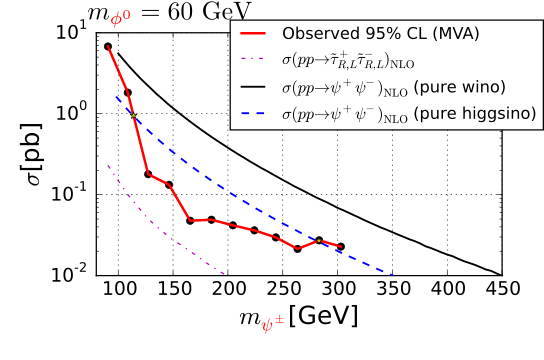
\includegraphics[scale=0.85]{tauMVA}}}    
% \only<2>{\put(-28,5){\includegraphics[scale=0.85]{tauMVA1}}}    
% \end{picture}
% \end{frame}

\begin{frame}
  \frametitle{ATLAS arXiv:1403.5294 (JHEP)}
  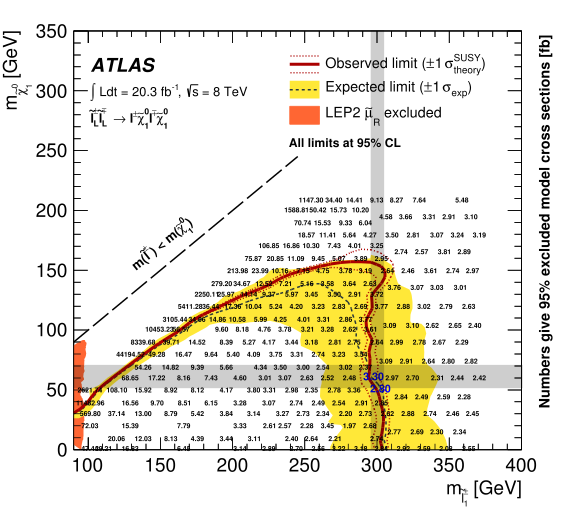
\includegraphics[scale=0.46]{figaux_20b} 
\parbox[b]{3cm}{
CMS\\
$\gtrsim 260$ GeV\\
arXiv:1405.7570 
}
\end{frame}

\begin{frame}
\frametitle{$m_{\phi^{0}}=60\ \text{GeV}$ }
\hspace{-1.4cm}\begin{overpic}[scale=0.8]{emuMVA}  
%%
%\includegraphics
\end{overpic}

\end{frame}




\section{Lepton flavor dependence}
\begin{frame}
  \frametitle{Neutrino masses}
  

\begin{align*}
  ({\mathcal{M}}_{\nu})_{\alpha\beta} =
\sum_{k=1}^{n_\Sigma} \left[{\color{red}Y^T} \Lambda {\color{red}Y}\right]_{\alpha\beta}~, \qquad  \alpha,\beta=1,2,3\,,
\end{align*}
From neutrino oscillation data, we can get a set of $\color{red}Y$ choosing the angles for $\color{red}R$, an arbitrary \emph{complex orthogonal matrix}
\begin{eqnarray}\label{eq:CasasIbarra}
{\color{red}Y} = \sqrt{\Lambda}^{-1} {\color{red}R}\;  
\operatorname{diag}( \sqrt{m_{\nu_{1}}}, \sqrt{m_{\nu_{2}}},\sqrt{m_{\nu_{3}}}  )
U_{\rm PMNS}^{\dagger}
\,,
\end{eqnarray}
\begin{align*}
{\color{red} \hat Y_{\alpha } } \equiv&\hat Y_{1\alpha} = {Y_{1\alpha}}/{ \sqrt{\sum_{\alpha=e,\mu,\tau} |Y_{1\alpha}|^2 }} &\hspace{0.5cm} {\color{red} \mathcal{B}_\alpha } \equiv &\operatorname{Br} (\Sigma_{1}^{\pm} \to \ell_\alpha H^{0}) = |{\color{red}\hat Y_\alpha}|^2\,.  
\end{align*}

Input parameters: \alert{3} complex angles and \alert{1} phase.
\end{frame}


\begin{frame}
  \frametitle{Casas-Ibarra parametrization}
In wino-like scotogenic model (may be in general)

\begin{picture}(320,170)
\only<1->{\put(-45,-10){\includegraphics[scale=0.4]{NH}}}    
\only<1->{\put(135,-10){\includegraphics[scale=0.4]{IH}}} 
\only<1->{\put(20,5){\scriptsize \alert{ Normal Hierarchy}}}
\only<1->{\put(200,5){\scriptsize \alert{ Inverted Hierarchy}}}
\only<2>{\put(35,130){
\includegraphics[scale=0.15]{highlight_circle}}}  \only<2>{\put(-30,2){
\includegraphics[scale=0.15]{highlight_circle}}}  
\only<2>{\put(108,2){
\includegraphics[scale=0.15]{highlight_circle}}}  
\end{picture}
\centering
$\mathcal{B}_l=\mathcal{B}\left( {\color{red}\Sigma^{\pm}}\to l^{\pm}{\color{red}H^0} \right)$ 
\end{frame}

\begin{frame}
  \frametitle{Exploration of flavor space}
\alert{Wino-like scotogenic model}: Recast for \alert{$B_{\mu}+B_e \gtrsim 0.1$} and
\begin{align*}
\color{red}  m_{H^0}<m_{\Sigma^{\pm}}= m_{\Sigma^{0}}<m_{A^0},m_{H^{\pm}}
\end{align*}

\vspace{-0.3cm}

Start with Signal regions as in ATLAS-arXiv:1403.5294 for\\


 $\cancel{E_T}$ with $e^+ e^-$, $\mu^+\mu^-$,
 $e^{\pm}\mu^{\mp}$. 

\centering
\texttt{SARAH/FeynRules} \\
$\Downarrow$\\
\texttt{micrOMEGAS} (Experimental and theoretical constraints) \\
$\Downarrow$\\
\texttt{MadGraph}\\
$\Downarrow$\\
\texttt{Pythia 6} (\texttt{hep} format)\\ 
$\Downarrow$\\
\texttt{checkMATE} (CL-calculation)
% \begin{align*}
%   CL=CL^{ee}CL^{\mu\mu}CL^{\mu e}
% \end{align*}
\end{frame}



\begin{frame}
  \frametitle{Combination}
  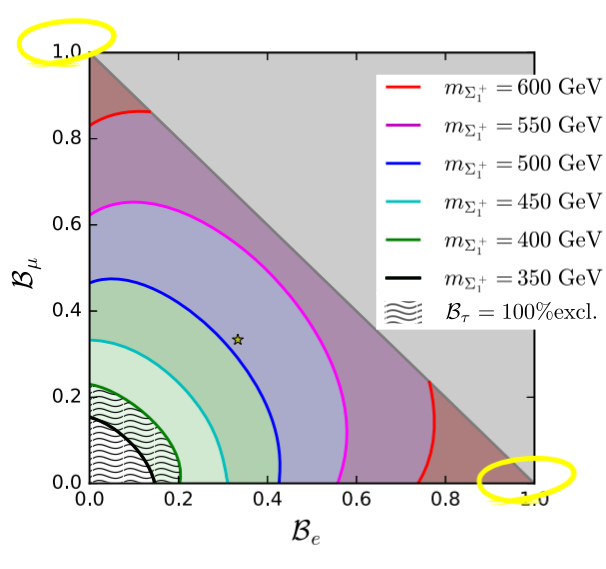
\includegraphics[scale=0.54]{clcomb}
\end{frame}

\section{Prospects for run-II}



\begin{frame}
  \frametitle{Golden EW SUSY channel: trilepton and $\cancel{E}_{T}$}
\begin{picture}(320,120)
  \only<1>{
\put(-30,123){\includegraphics[scale=0.36,angle=-90%
]{exclusion_TChiSlepSnu_2i_0_5}}%
\put(170,123){\includegraphics[scale=0.27,angle=-90%
]{CMS-PAS-SUS-16-024_Figure_007}}
}
  \only<2>{
\put(-30,123){\includegraphics[scale=0.36,angle=-90%
]{cms_quasi_dilepton_8TeV}}%
\put(170,123){\includegraphics[scale=0.27,angle=-90%
]{cms_quasi_dilepton_13TeV}}
}
\end{picture}

\vspace{0.5cm}

\only<1->{\small{ 
{\scriptsize arxiv:1405.7570 (8 TeV) \hfill SUS-16-024 (13 TeV)}\\
Improvement by a factor of $~1.4$\\

For a similar improvement we could expect exclusions at the level of \\
\alert{900~GeV in the wino-like scotogenic model,}

\alert{700 GeV in Higgsino-like scotogenic models.}

\alert{500 GeV in Bino-like scotogenic models.}
}
}

\end{frame}

\section{Vector-like fermion  mediation}

\begin{frame}
  \frametitle{Vector-like fermion mediation}
  Straightforward way to avoid DD constraints in scalar dark matter:

\rowcolors{1}{RoyalBlue!20}{RoyalBlue!5}
\begin{tabular}{LLLLLL}
\text{Name} & \text{Symbol} & \text{SU}(3)_c & \text{SU}(2)_L & \text{U}(1)_Y & Z_2  \\ %\hline
 \begin{pmatrix}\nu_L & e_L\end{pmatrix}^{\operatorname{T}}&
\begin{pmatrix}\xi_{1\alpha} & \xi_{2\alpha} \end{pmatrix}^{\operatorname{T}}& \mathbf{1} & \mathbf{2} & -1/2 & +1 \\
(e_R)^{\dagger} & \eta^{\alpha}_1 & \mathbf{1} & \mathbf{1} & +1 & +1 \\
\color{red}(\psi_R)^{\dagger} & \eta^{\alpha}_2 & \mathbf{1} & \mathbf{1} & +1 & -1 \\
\color{red}\psi_L & \xi_{3\alpha} & \mathbf{1} & \mathbf{1} & -1 & -1 \\
\color{blue}S & &  \mathbf{1} & \mathbf{1} & 0 & -1 \\
\end{tabular}
\begin{align*}
  \mathcal{L}\supset& y_e {\color{blue}S}  (e_R)^{\dagger} {\color{red}\psi_L}  + m_{\psi^{\pm}} {(\psi_R)^{\dagger}\color{red}\psi_L} 
 + \text{h.c} + \frac{1}{2}m_{S}{\color{blue}S^2} + \cancel{\lambda_{HS}S^2 H^{\dagger}H}%\underbrace{V({\color{blue}S})}_{\displaystyle m_S }
\end{align*}
See: arXiv:1307.6181 and arXiv:1307.6480
\end{frame}

\begin{frame}
  \frametitle{LHC constraints: Preliminary}
\includegraphics[scale=0.82]{singlet_exc}
\end{frame}

\begin{frame}
  \frametitle{Conclusions}
\emph{Opposite sign {\color{red}dilepton plus missing transverse energy } signal at LHC }

  The use of scotogenic models to interpret {\color{red}dilepton
plus missing transverse energy} searches, allow for larger sensitivities and 
full lepton flavor exploration

Additional motivation for fermion vectorlike mediation with {\color{red}zero three-level direct detection} cross section and challenging {\color{red}compressed spectra}.
\end{frame}

\plain{Thanks!}

\end{document}
\section{Recast at the LHC Run-I (wino-like scenario)}
\begin{frame}
  \frametitle{Exploration of flavor space}
\alert{Wino-like scotogenic model}: Recast for \alert{$B_{\mu}+B_e \gtrsim 0.1$} and
\begin{align*}
\color{red}  m_{H^0}<m_{\psi^{\pm}}= m_{\psi^{0}}<m_{A^0},m_{H^{\pm}}
\end{align*}

\vspace{-0.3cm}

Start with Signal regions as in ATLAS-arXiv:1403.5294 for\\


 $\cancel{E_T}$ with $e^+ e^-$, $\mu^+\mu^-$,
 $e^{\pm}\mu^{\mp}$. 

\centering
\texttt{FeynRules} \\
$\Downarrow$\\
\texttt{micrOMEGAS} (Experimental and theoretical constraints) \\
$\Downarrow$\\
\texttt{MadGraph}\\
$\Downarrow$\\
\texttt{Pythia 6} (\texttt{hep} format)\\ 
$\Downarrow$\\
\texttt{checkMATE} (CL-calcutation)
\begin{align*}
  CL=CL^{ee}CL^{\mu\mu}CL^{\mu e}
\end{align*}
\end{frame}
%region


% * <restrepo@udea.edu.co> 2015-11-15T17:13:36.188Z:
%
% Guillermo and Robinson Plot
%
% ^.
\begin{frame}
  \frametitle{ ATLAS arXiv:1509.07152, $X^+ X^-\to 2\times \tau\, \phi_{\rm{DM}}$: $X^+=\psi^+,{}^{\sim}\!\!\!\!{\tau}^+_{R,L}$ (MVA)}
\begin{picture}(320,250)
\only<1>{\put(-28,5){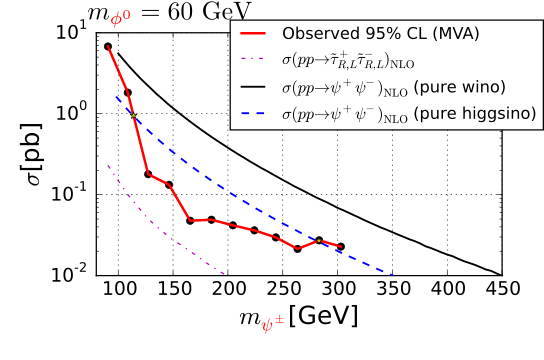
\includegraphics[scale=0.85]{tauMVA}}}    
\only<2>{\put(-28,5){\includegraphics[scale=0.85]{tauMVA1}}}    
\end{picture}
\end{frame}


% * <restrepo@udea.edu.co> 2015-11-15T17:13:36.188Z:
%
% ISR
%
% ^.
\begin{frame}
\frametitle{wino production to dilepton plus missing energy (ISR)}
\begin{picture}(320,250)
\only<1>{\put(-10,13){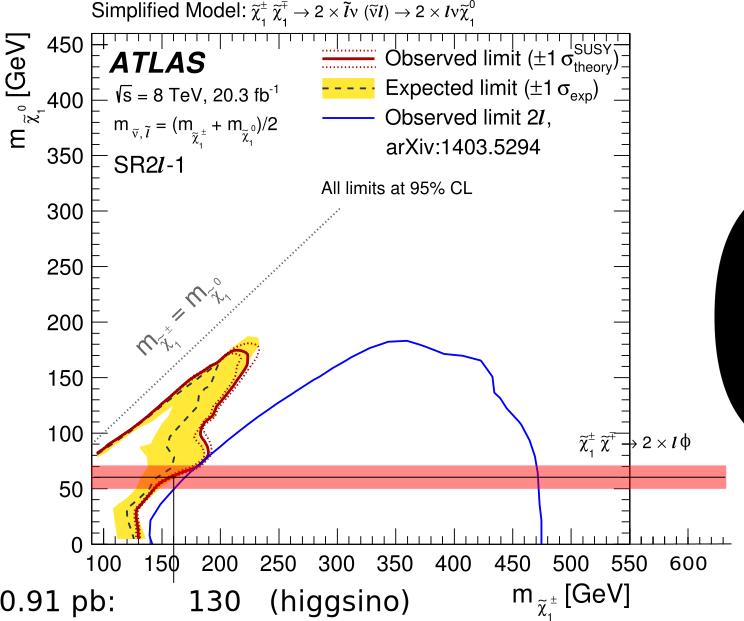
\includegraphics[scale=0.48]{fig_13b}}}    
\only<1>{ \put(240,180){ 
\parbox{3cm}{
$\color{blue}\overline{\hspace{0.5cm}}$ CMS\\
${m_{\tilde{\chi}_1^{\pm}}}\gtrsim 510$ GeV for\\
${m_{\tilde{\chi}_1^0}}< 100$ GeV\\
arXiv:1405.7570 \\
\quad\\
\small
$\color{red}\overline{\hspace{0.5cm}}$ CMS $\tilde{\chi}_1^{\pm}\tilde{\chi}_1^0$ \\
$\Delta M=20$ GeV (ISR)\\
\scriptsize
CMS-PAS-SUS-14-021
}
} }     
\end{picture}
\end{frame}

\begin{frame}
  \frametitle{Wino-like exclusion from Run-I}
\centering

  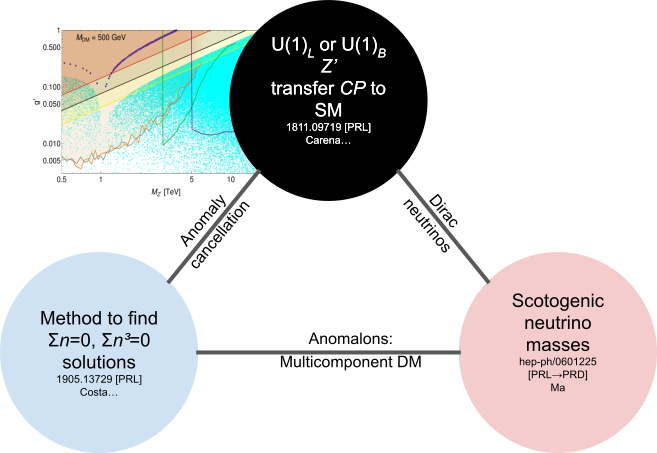
\includegraphics[scale=0.57]{triangle}
\end{frame}






\section{Conclusions}
% * <restrepo@udea.edu.co> 2015-11-15T17:13:36.188Z:
%
% Conlcusions: fill the gaps
%
% ^.
\begin{frame}[allowframebreaks]
  \frametitle{Conclusions}
\small
After give up the \alert{hierarchy problem} (\emph{heavy sfermion masses}),
\alert{dark matter} and \alert{gauge coupling unification} is not longer associated to SUSY
\begin{align*}
  \text{Bino-Higgsino-Wino} \underbrace{\longrightarrow}_{\text{generic couplings}} \color{red}\text{Singlet-Doublet-Triplet}
\end{align*}

But difficult to test at colliders, like radiative neutrino mass models

\vspace{-0.2cm}

\hrulefill

\vspace{-0.2cm}

$Z_{2}$-odd: {\color{red}Fermion(Singlet-Doublet-Triplet)+Scalar(Singlet-Doublet)}
\begin{itemize}
\item Radiative neutrino masses
\item Rich lepton flavor structure at low and high-energy experiments
\item Generic collider signal: dileptons plus 2$\times$($~60\ \text{GeV}$ DM.)
\end{itemize}

\alert{The wino-like scotogenic model}  (\emph{radiative type-III seesaw}) \alert{with $\mathcal{B}(\psi^+\to l_i \phi^0)=1$} is a a good simplified model for the interpretation of experimental results at the LHC.

\alert{At Run-I}, the charged fermion have been \alert{excluded} until \alert{630~GeV} (400 GeV)  for \alert{$\mathcal{B}(\psi^+\to e^+ \phi^0)=1$} $\left(\mathcal{B}(\psi^+\to \tau^+ \phi^0)=1 \right)$, 

\alert{Including the compressed-spectra region}

\emph{TODO: Higgsino-like case}
\end{frame}







\begin{frame}[plain]
  \begin{picture}(320,250)
    \only<1>{\put(-27,-10){\includegraphics[scale=0.44]{dmwmodelsnew1}}}
    \only<1>{\put(110,180){
      \begin{minipage}[t]{0.65\linewidth}
            %\metroset{block=fill}
            \begin{alertblock}{Type-I RS \texttt{SARAH} implementation}
             \quad

             arXiv:1507.06349 by \textit{Avelino Vicente}
             
             Slides and Code \@ 

             {\scriptsize\url{https://github.com/restrepo/Scotogenic}}
              
            \end{alertblock}

      \end{minipage}
}
}
    \only<2>{\put(-27,-10){\includegraphics[scale=0.44]{dmwmodelsnew2}}}
    \only<3>{\put(-27,-10){\includegraphics[scale=0.44]{dmwmodelsnew3}}}
    \only<4>{\put(-27,-10){\includegraphics[scale=0.44]{dmwmodelsnew4}}}
    \only<5>{\put(-27,-10){\includegraphics[scale=0.44]{dmwmodelsnew5}}}
\end{picture}
\end{frame}



\begin{frame}
\begin{picture}(320,250)
\only<1>{\put(-30,-10){\includegraphics[scale=0.8]{excl4}}}    
\end{picture}
\end{frame}
% * <restrepo@udea.edu.co> 2015-11-15T17:13:36.188Z:
%
% Guillermo and Robinson Plot region
%
% ^.
\begin{frame}
\begin{picture}(320,250)
\only<1>{\put(-30,-10){\includegraphics[scale=0.8]{excl5}}}    
\end{picture}
\end{frame}


\section{Beyond the standard model}

\begin{frame}\frametitle{Recover fundamental masses \frownie{}}
%\metroset{block=fill}
  \begin{block}{Singlet scalar dark matter}
    \begin{align*}
      Z_2:\qquad \mathcal{L}_{\text{SM}}\to \mathcal{L}_{\text{SM}}\,,\qquad
           S\to -S\,.
    \end{align*}
    \begin{align*}
      \mathcal{L}=\mathcal{L}_{\text{SM}}+\frac{1}{2}\partial_{\mu}S\partial^{\mu}S-\frac{1}{2} {\color{red}m_S^2}S^{2}-\frac{1}{4}\lambda S^4\,+{\color{blue}\lambda_{SH}} \Phi^{\dagger}\Phi S^2.
    \end{align*}

  \end{block}
  \begin{block}{Singlet fermion: Seesaw}
    \begin{align*}
      \mathcal{L}=&\mathcal{L}_{\text{SM}}+ i N^{\dagger}\overline{\sigma}^{\mu}\partial_{\mu}N+  \left( h_{\nu}L\cdot\Phi N-{\color{red}M}\; N N+\text{h.c} \right)\,,&&\nonumber\\
&m_1\sim \frac{h_{\nu}v^2}{\sqrt{2} {\color{red}M}}\,,& m_2\sim& {\color{red}M}\,.
    \end{align*}
\centering
${\color{red}M}\gg h_{\nu}v/\sqrt{2}$
  \end{block}
\end{frame}

\begin{frame}[fragile]
  \frametitle{SARAH implementation}
  \begin{itemize}
  \item<1->   Automatic generation of \texttt{Fortran-90} \alert{\texttt{SPheno}} code and interaction-basis Les-Houches Accord \alert{(LHA) input file}, for calculation of: 
   \begin{itemize}
  \item  1-loop spectrum
  \item  Decay branching (including generic one loop $S\to \gamma\gamma,GG$)
  \item LFV observables
  \item LHA output 
  \end{itemize}
\item<2-> Automatic generation of model files through \alert{LHA \texttt{SPheno} output} for
  \begin{itemize}
  \item \alert{\texttt{CalcHEP}} 
  \item \alert{\texttt{micrOMEGAS}}
  \item \alert{\texttt{MadGRAPH}}
  \item \alert{$\boldsymbol{\cdots}$}
  \end{itemize}
\item<3> \textbf{Hint}: Use \alert{\texttt{SARAH Toolbox}} toolkit: {\tiny \url{https://sarah.hepforge.org/Toolbox.html}} 
\begin{verbatim}
$  ./butler SSDM #Your model name
\end{verbatim}
  \end{itemize}
\end{frame}

\begin{frame}[fragile,allowframebreaks]
  \frametitle{SSDM in SARAH-}
\url{./SARAH/Models/SSDM/SSDM.m}
  \begin{itemize} 
  \item<1> \footnotesize
\begin{verbatim}
Global[[1]] = {Z[2], Z2};
Gauge[[1]]={B,   U[1], hypercharge, g1,False,1};
Gauge[[2]]={WB, SU[2], left,        g2,True,1};
Gauge[[3]]={G,  SU[3], color,       g3,False,1};

FermionFields[[1]] = {q, 3, {uL, dL},     1/6, 2,  3,1};  
FermionFields[[2]] = {l, 3, {vL, eL},    -1/2, 2,  1,1};
FermionFields[[3]] = {d, 3, conj[dR],     1/3, 1, -3,1};
FermionFields[[4]] = {u, 3, conj[uR],    -2/3, 1, -3,1};
FermionFields[[5]] = {e, 3, conj[eR],       1, 1,  1,1};
ScalarFields[[1]] =  {H, 1, {Hp, H0},     1/2, 2,  1,1};
ScalarFields[[2]] =  {S, 1, ss,     0, 1,  1, -1};
RealScalars = {S};
\end{verbatim}
  \item<2> \footnotesize
\begin{verbatim}
...
NameOfStates={GaugeES, EWSB};

DEFINITION[GaugeES][LagrangianInput]= {
	{LagHC, {AddHC->True}},
	{LagNoHC,{AddHC->False}}
};


LagNoHC = -(mu2 conj[H].H + Lambda1/2 conj[H].H.conj[H].H 
            + MS2/2 S.S + LamSH S.S.conj[H].H  
            + LamS/2 S.S.S.S);
LagHC =  -(Yu H.u.q+Yd conj[H].d.q + Ye conj[H].e.l);

\end{verbatim}
  \item<2> \footnotesize
\begin{verbatim}
DEFINITION[EWSB][GaugeSector] =
{ 
  {{VB,VWB[3]},{VP,VZ},ZZ},
  {{VWB[1],VWB[2]},{VWp,conj[VWp]},ZW}
};     

DEFINITION[EWSB][VEVs]= 
{{H0, {v, 1/Sqrt[2]}, {Ah, I/Sqrt[2]},{hh, 1/Sqrt[2]}}     };

DEFINITION[EWSB][MatterSector]=   
    {{{{dL}, {conj[dR]}}, {{DL,Vd}, {DR,Ud}}},
     {{{uL}, {conj[uR]}}, {{UL,Vu}, {UR,Uu}}},
     {{{eL}, {conj[eR]}}, {{EL,Ve}, {ER,Ue}}}};  

DEFINITION[EWSB][DiracSpinors]={
 Fd ->{  DL, conj[DR]}, ...
\end{verbatim}
  \end{itemize}
\end{frame}



\section{Dark matter and unification}

\begin{frame}
  \frametitle{Unification: $SO(10)$}
  \begin{columns}
    \begin{column}{0.7\textwidth}
      \begin{small}
  \begin{align*}
    \mathbf{16}_{F_{i}}=
    \begin{pmatrix}
      {{\color{green}u_{R}}^{\dagger}}\\
      {{\color{blue}u_{R}}^{\dagger}}\\
      {{\color{red}u_{R}}^{\dagger}}\\
      {{\color{green}u_{L}}}\\
      {{\color{blue}u_{L}}}\\
      {{\color{red}u_{L}}}\\
      {{\color{green}d_{L}}}\\
      {{\color{blue}d_{L}}}\\
      {{\color{red}d_{L}}}\\
      {{\color{green}d_{R}}^{\dagger}}\\
      {{\color{blue}d_{R}}^{\dagger}}\\
      {{\color{red}d_{R}}^{\dagger}}\\
      \nu_L\\
      e_L\\
      {e_{R}}^{\dagger}\\
      N\\
    \end{pmatrix}_{i} \qquad\Rightarrow \mathcal{L}_{SM}\supset h\, \mathbf{16}_F\times\mathbf{16}_{F}\times \mathbf{10}_{S}+\text{h.c}
  \end{align*}
      \end{small}
    \end{column}
    \begin{column}{0.3\textwidth}
  \hfill\includegraphics[scale=0.2]{sym}      
    \end{column}
  \end{columns}


\end{frame}


\begin{frame}
\frametitle{Not-susy $\operatorname{SO}(10)\to SU(5)\to \operatorname{SU}(3)_C\times SU(2)_L \times \operatorname{U}(1)_Y \times Z_2 $}
\begin{picture}(320,250)
%\includegraphics[scale=0.2]{tocrs}
 %   
 % \only<1->{\put(-11,10){\includegraphics[scale=0.4]{tocrs}}}%
 % 
 \only<1->{\put(-10,250){
  \begin{columns}[T,onlytextwidth]
    \column{0.5\textwidth}
      %\metroset{block=fill}
      \begin{block}{Standard Model: $Z_2$-even }
        Fermions: $\boldsymbol{16}_F$

        Scalars: $\boldsymbol{10}_H,\boldsymbol{45}_H\cdots$
      \end{block}


    \column{0.5\textwidth}

      %\metroset{block=fill}


      \begin{alertblock}{New $Z_2$-odd particles}
       \color{red}
        $\boldsymbol{10}_F,\boldsymbol{45}_F,\cdots$
       
        $\boldsymbol{16}_H,\cdots$
      \end{alertblock}
  \end{columns}
}
}
\only<1->{\put(-10,200){
    \begin{minipage}[t]{1.0\textwidth}
 \alert{Lightest Odd Particle (LOP)} may be  a suitable dark matter candidate, \alert{and can improve gauge coupling unification }
    \end{minipage}
}
}
\only<1>{\put(0,20){
\includegraphics[scale=0.45]{smunif}
}
}
\only<2->{\put(0,90){
  \begin{overpic}[height=3cm%,grid
            ]{table1}
\put(16,0){\tikz \draw[red,thick,rounded corners,fill=orange,fill opacity=0.2] (0,0) rectangle (0.5,0.5);}
\put(62,0){\tikz \draw[red,thick,rounded corners,fill=orange,fill opacity=0.2] (0,0) rectangle (0.5,0.5);}
\put(38,-7){\tikz \draw[red,thick,rounded corners,fill=orange,fill opacity=0.2] (0,0) rectangle (1.,0.5);}
\only<5>{\put(18,-7){\tikz \draw[red,thick,rounded corners,fill=orange,fill opacity=0.2] (0,0) rectangle (0.9,0.5);}}
\only<3->{\put(16,6){\tikz \draw[green,thick,rounded corners,fill=green,fill opacity=0.2] (0,0) rectangle (1.,0.5);}}
\only<3->{\put(50,6){\tikz \draw[green,thick,rounded corners,fill=green,fill opacity=0.2] (0,0) rectangle (0.5,0.5);}}
\only<3-4>{\put(16,13){\tikz \draw[blue,thick,rounded corners,fill=blue,fill opacity=0.2] (0,0) rectangle (0.5,0.5);}}
\only<3-4>{\put(55,13){\tikz \draw[blue,thick,rounded corners,fill=blue,fill opacity=0.2] (0,0) rectangle (0.5,0.5);}}
\only<5>{\put(16,13){\tikz \draw[orange,thick,rounded corners,fill=orange,fill opacity=0.2] (0,0) rectangle (0.5,0.5);}}
\only<4->{\put(30,5){\tikz \draw[black,thick,rounded corners,fill=black,fill opacity=0.2] (0,0) rectangle (1.,0.6);}}
\only<4->{\put(32,8){\parbox[t]{2cm}{$\mathbf{2}_{1/2}^{S}$}}}
  \end{overpic}
  \begin{overpic}[height=3cm%,grid
            ]{table2}
\only<4->{\put(30,30){\tikz \draw[black,thick,rounded corners,fill=black,fill opacity=0.2] (0,0) rectangle (0.5,0.5);}}
  \end{overpic}
}
}
\only<2-5>{\put(0,80){
  \begin{minipage}[t]{1.0\linewidth}
    $SU(3)_{C}: \mathbf{3}\; (T),\ \mathbf{6},\ \mathbf{8}\;(\Lambda) $
  \end{minipage}
}
%\put(40,38){\color{red}${}^{2}$}
}
\only<2>{\put(0,70){
  \begin{minipage}[t]{1.0\linewidth}
    \begin{align*}
      m_{3_0}=2.7\ \text{TeV},\qquad m_{\Lambda}\sim 10^{10}\ \text{TeV},\qquad m_{\text{GUT}}\sim 10^{16}\ \text{GeV}\,.
    \end{align*}
    arXiv:0912.1545 (Frigerio-Hambye)
  \end{minipage}
}
}
\only<3>{\put(0,70){
  \begin{minipage}[t]{1.0\linewidth}
\centering
     \alert{Split-SUSY like}

    %uniftwo451E16
    arXiv:1509.06313 (C. Arbelaez, R. Longas, D.R, O. Zapata)
  \end{minipage}
}
}
%%%circle
\invisible<1-3>{\put(0,82){      %\metroset{block=fill}
    \begin{minipage}[t]{1.0\linewidth}
      \begin{exampleblock}{\only<4>{Radiative hybrid seesaw (Parida {%\tiny 
1106.4137}) or} 1509.06313}
      \centering
      \only<4>{Partial  Split-}SUSY-like spectrum: {\color{red}bino}-higgsino-{\color{red}wino}

               \hfill             + $\color{red}\hspace{3cm}\downarrow$\hspace{3cm}    
        
         $\boldsymbol{10}'_H$ with fermion DM or, \hspace{0.5cm}  \color{red}
         $\boldsymbol{16}_H,\cdots$ with scalar DM 
        
      \end{exampleblock}
    \end{minipage}
}
}
\end{picture}


\end{frame}
\begin{frame}
  \frametitle{{\color{red}Singlet-Doublet}-Triplet fermion dark-matter}
The most general $\text{SO}(10)$ invariant Lagrangian contains the following Yukawa terms
\begin{align*}
-\mathcal{L} & \supset  Y{\bf 10}_F {\bf 45}_F {\bf 10}_H + M_{\mathbf{45}_F}{\bf 45}_F{\bf 45}_F + M_{\mathbf{10}_F}{\bf 10}_F{\bf 10}_F
\invisible<1>{+{\mathcal{L}(\alert{\mathbf{10}_\Phi}\invisible<2>{\ \text{or}\   \mathbf{16}_\Phi})}.} 
\end{align*}



  \begin{columns}
    \begin{column}{0.47\textwidth}
Basis $\boldsymbol{\psi}^0=\left({\color{red}N},\Sigma^0,{\color{red}\psi_L^0},{\color{red}\left( \psi_R^0 \right)^{\dagger}}\right)^T$ 
\tiny
\begin{align*}
  &\mathcal{M}_{\boldsymbol{\psi}^0}=\nonumber\\
&\begin{pmatrix}
{\color{red}M_N}          &   0       &{\color{red}-y\,c_\beta v/\sqrt{2}}&{\color{red}y\,s_\beta v/\sqrt{2}} \\
0 & M_\Sigma &  f\,c_{\beta'}v/\sqrt{2} & -f\,s_{\beta'}v/\sqrt{2}\\
{\color{red}-y\,c_\beta} v/\sqrt{2} &  f\,c_{\beta'}v/\sqrt{2}  & 0            & {\color{red}}-M_D\\
{\color{red}y\,s_\beta v/\sqrt{2}}& -f\,s_{\beta'}v/\sqrt{2}&{\color{red}}  -M_D                &  0  \\
\end{pmatrix},
\end{align*}
    \end{column}
    \begin{column}{0.53\textwidth}
      \only<2>{\includegraphics[scale=0.38]{rumor}}
      \only<3>{\includegraphics[scale=0.38]{sdfdm}}
    \end{column}
  \end{columns}

  \invisible<2->{Model used for the Nimatron proposal: arXiv:1511.06495\\
{\small \textbf{Physics Opportunities of a 100 TeV Proton-Proton Collider}\\
Nima Arkani-Hamed, T. Han, M. Mangano, LT Wang. }
}
\end{frame}
\begin{frame}
  \frametitle{Split-SUSY like}
\centering

  \includegraphics[scale=0.8]{uniftwo451E16}
\end{frame}

\begin{frame}
  \frametitle{Partial split-SUSY like}
\centering

  \includegraphics[scale=0.8]{uniftwo452E3}
\end{frame}

\begin{frame}
  \frametitle{SUSY like}
\begin{picture}(320,250)
\put(-40,100){ \includegraphics[scale=0.5]{unif2E3}  }
\put(125,100){\includegraphics[scale=0.5]{unif1E10} }
\end{picture}
\end{frame}



\begin{frame}
  \frametitle{Weinberg operator at one-loop}
\begin{textblock*}{297mm}(68mm,0.5mm)%
\begin{beamercolorbox}[sep=0.01em,wd=5.7cm,center,rounded=true,shadow=true]{cite}
\scriptsize Bonnet, Hirsch, Ota, Winter, arXiv:1204.5862 (JHEP)
\end{beamercolorbox}
\end{textblock*}

  \begin{block}{Notations}
    \begin{center}
      \begin{align*}
        \alert{\mathbf{X}}^{\color{OliveGreen}\mathcal{L}}_{\color{blue}\mathbf{Y}}
      \end{align*}
      \begin{itemize}
      \item $\color{OliveGreen}\mathcal{L}$ Lorentz nature: scalar ($\color{OliveGreen}S$) or fermion ($\color{OliveGreen}F$),
      \item $\color{blue}Y\equiv 2(Q-I_3)$ hypercharge: $\color{blue}\alpha$ arbitrary rational-number
      \item $\alert{\mathbf{X}}$ $SU(2)$ nature: singlet $\alert{\mathbf{1}}$, doublet $\alert{\mathbf{2}}$, triplet $\alert{\mathbf{3}}$
        \begin{itemize}
        \item quadruplet $\alert{\mathbf{4}}$, quintuplet $\alert{\mathbf{5}}$, $\ldots$ \begin{beamercolorbox}[sep=0.01em,wd=5.7cm,center,rounded=true,shadow=true]{cite}
\scriptsize Law, McDonald, arXiv:1305.6467
\end{beamercolorbox}

        \end{itemize}

      \end{itemize}
    \end{center}
  \end{block}
\end{frame}
%%%%%%%%%%%%%%%%%%%%%%%%%%%%%%
\begin{frame}
\frametitle{Weinberg operator at one-loop}
\only<1>{\begin{textblock*}{297mm}(68mm,0.5mm)%
\begin{beamercolorbox}[sep=0.01em,wd=5.7cm,center,rounded=true,shadow=true]{cite}
\scriptsize Ma, hep-ph/9805219 (PRL)
\end{beamercolorbox}
\end{textblock*}
}%  
\only<2->{\begin{textblock*}{297mm}(68mm,0.5mm)%
\begin{beamercolorbox}[sep=0.01em,wd=5.7cm,center,rounded=true,shadow=true]{cite}
\scriptsize Bonnet, Hirsch, Ota, Winter, arXiv:1204.5862 (JHEP)
\end{beamercolorbox}
\end{textblock*}
}%  
\begin{picture}(320,250)
\only<2->{\put(0,140){\includegraphics[scale=0.8]{T1-1}}}%
\only<1->{\put(180,140){\includegraphics[scale=0.8]{T1-2}}}%
\only<1->{\put(0,20){\includegraphics[scale=0.8]{T3}}}%
\only<1->{\put(180,20){\includegraphics[scale=0.8]{T1-3}}}%
\only<2>{\put(170,5){and reducible and divergent topologies}}%
\only<3->{\put(40,110){\fcolorbox{black}{blue}{\color{white}Radiative seesaw}
}}%
\only<3->{\put(80,25){\color{red}\circle{12}}}%
\only<3->{\put(0,6){\fbox{$\alert{1}^{F}_{\color{blue}1+\alpha}\,,
\alert{2}^{F}_{\color{blue}1+\alpha}\,,
\alert{3}^{F}_{\color{blue}1+\alpha}\,,
\alert{4}^{F}_{\color{blue}1+\alpha}\,,
\alert{5}^{F}_{\color{blue}1+\alpha}\,,\cdots$}}}%
\only<4->{\put(233,186){\fcolorbox{black}{blue}{\color{white}Zee model}
}}%
\end{picture}
\end{frame}
%%%%%%%%%%%%%%%%%%%%%%%%%%%%%%

\begin{frame}\frametitle{Generalized Zee model}
\begin{picture}(320,250)
%%%REFERENCES
\only<1>{\put(150,250){\begin{beamercolorbox}[sep=0.01em,wd=6cm,center,rounded=true,shadow=true]{cite}
\scriptsize A. Zee, Phys.Lett.B93(1980)389 .
\end{beamercolorbox}%
}}%
\only<2>{\put(150,250){\begin{beamercolorbox}[sep=0.01em,wd=6cm,center,rounded=true,shadow=true]{cite}
\scriptsize E. Ma, hep-ph/9805219 (PRL)
\end{beamercolorbox}%
}}%
\only<3>{\put(150,250){\begin{beamercolorbox}[sep=0.01em,wd=6cm,center,rounded=true,shadow=true]{cite}
\scriptsize Bonnet, Hirsch, Ota, Winter, arXiv:1204.5862 (JHEP)
\end{beamercolorbox}%
}}%
\only<4>{\put(150,250){\begin{beamercolorbox}[sep=0.01em,wd=6cm,center,rounded=true,shadow=true]{cite}
\scriptsize [?]
\end{beamercolorbox}%
}}%
\only<5->{\put(150,250){\begin{beamercolorbox}[sep=0.01em,wd=6cm,center,rounded=true,shadow=true]{cite}
\scriptsize D.R, Yagunga, Zapata,  arXiv:1308.3655
\end{beamercolorbox}%
}}%

\only<1->{\put(2,160){\includegraphics[scale=0.7]{T1-2}%
}}
\put(145,120){\renewcommand{\arraystretch}{1.3}
\rowcolors{1}{RoyalBlue!20}{RoyalBlue!5}
  \begin{tabular}{p{1.1cm}|p{1.1cm}|p{1.1cm}|p{1.1cm}|p{0.5cm}}
    $\psi$ & $\phi$ & $\phi'$ & $\psi'$&\only<5->{$\alpha$}\\
%row2
\only<3-4>{$\alert{1^F_\alpha}$}    \only<5->{$\alert{\mathbf{1}^F_0}$}    &%
\only<3-4>{$\alert{2^S_{1+\alpha}}$}\only<5->{$\alert{\mathbf{2}^S_{1}}$}&%
\only<3-4>{$\alert{1^S_\alpha}$}    \only<5->{$\alert{\mathbf{1}^S_0}$}    &%
\only<3-4>{$\alert{2^F_{1+\alpha}}$}\only<5->{$\alert{2^F_{1}}$}&%
\only<6>{\fbox{$0$}}\only<7->{$0$}\\
%row 4
\only<1>{$2^F_1\text{:}\;\overline{e_{L}}$}%
\only<2-4>{$\alert{2^F_\alpha}$}
\only<5->{$\alert{2^F_{-1}}$}&%
\only<1>{$1^S_2\text{:}\;\eta^+$}%
\only<2-4>{$\alert{1^S_{1+\alpha}}$}%
\only<5->{$\alert{1^S_{-2}}$}&%
\only<1>{$2^S_1\text{:}\;\phi$}%
\only<2-4>{$\alert{2^S_\alpha}$}%
\only<5->{$\alert{\mathbf{2}^S_{-1}}$}&%
\only<1>{$1^F_2\text{:}\;\overline{e_{R}}$}%
\only<2-4>{$\alert{1^F_{1+\alpha}}$}%
\only<5->{$\alert{1^F_{-2}}$}&%
\only<7>{\fbox{$-2$}}\only<8->{$-2$}\\ 
%row3
\only<3-4>{$\color{blue}1^F_\alpha$}%
\only<5->{$\color{blue}\mathbf{1}^F_0$}&%
\only<3-4>{$\color{blue}2^S_{1+\alpha}$}%
\only<5->{$\color{blue}\mathbf{2}^S_{1}$}&%
\only<3-4>{$\color{blue}3^S_\alpha$}%
\only<5->{$\color{blue}{3}^S_0$}&%
\only<3-4>{$\color{blue}2^F_{1+\alpha}$}%
\only<5->{$\color{blue}2^F_{1}$}&%
\only<6>{\fbox{$0$}}\only<7->{$0$}\\ 
%row6
\only<2-4>{$\color{blue}2^F_\alpha$}%
\only<5->{$\color{blue}2^F_{-1}$}&%
\only<2-4>{$\color{blue}3^S_{1+\alpha}$}%
\only<5->{$\color{blue}3^S_{-2}$}&%
\only<2-4>{$\color{blue}2^S_\alpha$}%
\only<5->{$\color{blue}\mathbf{2}^S_{-1}$}&%
\only<2-4>{$\color{blue}1^F_{1+\alpha}$}%
\only<5->{$\color{blue}1^F_{-2}$}&%
\only<7>{\fbox{$-2$}}\only<8->{\fbox{$\mathbf{-2}$}}\\ 
%row7
\only<2-4>{$\color{OliveGreen}2^F_\alpha$}%
\only<5->{$\color{OliveGreen}2^F_1$}&%
\only<2-4>{$\color{OliveGreen}3^S_{1+\alpha}$}%
\only<5->{$\color{OliveGreen}3^S_{2}$}&%
\only<2-4>{$\color{OliveGreen}2^S_\alpha$}%
\only<5->{$\color{OliveGreen}\mathbf{2}^S_1$}&%
\only<2-4>{$\color{OliveGreen}3^F_{1+\alpha}$}%
\only<5->{$\color{OliveGreen}3^F_{2}$}&%
\only<7>{\fbox{$1$}}\only<8->{\fbox{$\mathbf{1}$}}\\ 
%row9
\only<3-4>{$\color{OliveGreen}3^F_\alpha$}%
\only<5->{$\color{OliveGreen}\mathbf{3}^F_0$}&%
\only<3-4>{$\color{OliveGreen}2^S_{1+\alpha}$}%
\only<5->{$\color{OliveGreen}\mathbf{2}^S_{-1}$}&%
\only<3-4>{$\color{OliveGreen}3^S_\alpha$}%
\only<5->{$\color{OliveGreen}\mathbf{3}^S_0$}&%
\only<3-4>{$\color{OliveGreen}2^F_{1+\alpha}$}%
\only<5->{$\color{OliveGreen}2^F_{-1}$}&%
\only<6>{\fbox{$-1$}}\only<7->{$-1$}\\  
%row 5
\only<2-4>{$2^F_\alpha$}%
\only<5->{$2^F_1$}&%
\only<2-4>{$1^S_{1+\alpha}$}%
\only<5->{$1^S_{2}$}&%
\only<2-4>{$2^S_\alpha$}%
\only<5->{$\mathbf{2}^S_1$}&%
\only<2-4>{$3^F_{1+\alpha}$}%
\only<5->{$3^F_{2}$}&%
\only<7>{\fbox{$1$}}\only<8->{\fbox{$\mathbf{1}$}}\\ 
%row8
\only<3-4>{$3^F_\alpha$}%
\only<5->{$\mathbf{3}^F_0$}&%
\only<3-4>{$2^S_{1+\alpha}$}%
\only<5->{$\mathbf{2}^S_{-1}$}&%
\only<3-4>{$1^S_\alpha$}%
\only<5->{$\mathbf{1}^S_0$}&%
\only<3-4>{$2^F_{1+\alpha}$}%
\only<5->{$2^F_{-1}$}&%
\only<6>{\fbox{$-1$}}\only<7->{$-1$}\\ 
\multicolumn{4}{c}{\only<4->{Larger $SU(2)_L$ multiplets}}&%
\\
  \end{tabular}%
}%
\only<3>{\put(20,80){\huge$\alert{\alpha\to-\alpha-1}$}}%
\only<5>{\put(-20,170){\parbox[t]{6cm}{
      \begin{center}
        \textbf{Dark matter filter}
      \end{center}
\vspace{-0.5cm}

      \begin{itemize}
      \item Impose $Z_2$ symmetry
        \begin{itemize}
        \item SM particles are even
        \item New particles are odd
        \end{itemize}
      \item Lightest odd particle (LOP)
        \begin{itemize}
        \item Color and electrically neutral
        \item Consistent with direct detection constraints
        \end{itemize}
      \item Odd fermions must be vector-like
      \end{itemize}
}}}%
\only<5>{\put(10,10){\fcolorbox{black}{blue}{\color{white}$Y=-2T_3$ for at least one particle}%
}}%
\only<6>{\put(0,100){\begin{beamercolorbox}[sep=0.1em,wd=4.7cm,center,rounded=true,shadow=true]{white}
\alert{Radiative type-I/III seesaw } with
additional contribution to neutrino masses.
\end{beamercolorbox}
}}%
\only<6>{\put(2,10){\includegraphics[scale=0.7]{T3}}
}%
\only<7-8>{\put(0,100){\begin{beamercolorbox}[sep=0.1em,wd=4.7cm,center,rounded=true,shadow=true]{white}
\alert{Inert doublet model} with
 one-loop neutrino masses (susy-like)
\end{beamercolorbox}
}}%
\only<8>{\put(0,60){\begin{beamercolorbox}[sep=0.1em,wd=4.7cm,center,rounded=true,shadow=true]{white}
and exotic charges
\end{beamercolorbox}
}}

\end{picture}  
\end{frame}
%%%%%%%
%%%%%%%%%%%%%%%%%%%%%%%%
\begin{frame}[plain]
\begin{picture}(320,250)
\only<1>{\put(-12,-13){\includegraphics[width=\paperwidth,height=\paperheight]{dmwmodels1}}}%
\only<2>{\put(-12,-13){\includegraphics[width=\paperwidth,height=\paperheight]{dmwmodels2}}}%
\only<3>{\put(-12,-13){\includegraphics[width=\paperwidth,height=\paperheight]{dmwmodels3}}}%
\only<4>{\put(-12,-13){\includegraphics[width=\paperwidth,height=\paperheight]{dmwmodels4}}}%
\only<5>{\put(-12,-13){\includegraphics[width=\paperwidth,height=\paperheight]{dmwmodels5}}}%
\only<6>{\put(-12,-13){\includegraphics[width=\paperwidth,height=\paperheight]{dmwmodels6}}}%
\only<7>{\put(-12,-13){\includegraphics[width=\paperwidth,height=\paperheight]{dmwmodels7}}}%
\only<8>{\put(-12,-13){\includegraphics[width=\paperwidth,height=\paperheight]{dmwmodels8}}}%
\only<9>{\put(-12,-13){\includegraphics[width=\paperwidth,height=\paperheight]{dmwmodels9}}}%
\only<10>{\put(-12,-13){\includegraphics[width=\paperwidth,height=\paperheight]{dmwmodels10}}}%
\only<10>{\put(40,240){\begin{beamercolorbox}[sep=0.01em,wd=5.7cm,center,rounded=true,shadow=true]{cite}
\scriptsize Law, McDonald, arXiv:1305.6467
\end{beamercolorbox}}}
\end{picture}
\end{frame}
%%%%%%%%%%%%%%%%%%%%%%%
\begin{frame}
\begin{picture}(320,250)
\only<1>{\put(-10,98){\includegraphics[scale=0.5]{09074193}}}%
\only<1>{\put(20,238){\small arXiv:0907.4193:  $3^{F}_{0}$}}%
\only<1>{\put(150,98){\includegraphics[scale=0.6]{13034404}}}%
\only<1>{\put(160,238){\small arXiv:1303.4404:  $2^{F,S}_{\pm 1}$ (solid) $1^{F,S}_{\pm 2}$ (dashed)}}%
\only<1>{\put(100,-20){\includegraphics[scale=0.72]{12013764}}}%
\only<1>{\put(10,40){\small arXiv:1201.3764  $3^{F}_{\pm 2}$}}%

\end{picture}
\end{frame}
%%%%%%%%%%%%%%%%
\begin{frame}
\begin{picture}(320,250)
\only<1>{\put(-10,70){\includegraphics[scale=0.5]{12022014}}}%
\only<1>{\put(20,60){\small arXiv:1202.2014:  $3^{S}_{\pm 2}$}}%
\only<1>{\put(150,0){\includegraphics[scale=0.6]{08113957}}}%
\only<1>{\put(180,0){\small arXiv:0811.3957:  $3^{S}_{0}$}}%

\end{picture}
\end{frame}

%\begin{frame}
%Phys Rev D85 095018
%\begin{picture}(320,250)
%\only<1>{\put(-10,70){\includegraphics[scale=0.5]{12022014}}}%
%\only<1>{\put(20,40){\small arXiv:1202.2014:  $3^{S}_{\pm 2}$}}%
%\end{picture}
%\end{frame}



%%%%%%%%%%%
\begin{frame}
  \frametitle{Discussion}
\includegraphics[scale=0.6]{alg}
  \begin{itemize}
  \item The collider and dark matter phenomenology  of many of these viable models have yet to be studied in detail.
  \item We have only qualitatively described the particle content and the dark matter candidates of each model. A more specific analysis of some of these models is certainly desirable.
\item Some strategies to systematically search for this kind of models
  at colliders would be designed. 
  \item New particles allowed to be even under $Z_2$ could give rise to new possibilities.
  \end{itemize}
\end{frame}
%%%%%%%%%%%%%%%%5

\begin{frame}
  \frametitle{Higgsino-like radiative seesaw}
  \begin{align*}
    10\times 16=&16+144 \nonumber\\
    \overline{16}\times 16=1+\cdots \nonumber\\
    \overline{144}\times 144=1+\cdots
  \end{align*}
The singlet comes from the following $SU(5)$ representation
\begin{align*}
      \overline{144}\times 144\supset 24\times24=1
\end{align*}
and the singlet can be choosen real
\end{frame}





\section{New simplified models}
% * <restrepo@udea.edu.co> 2015-11-15T12:41:09.269Z:
%
% One-loop diagrams with the  1-loop examples
%
% One-loop diagrams with the  1-loop examples
%
% ^.

% * <restrepo@udea.edu.co> 2015-11-15T12:43:05.091Z:
%
% two-loop example
%
% ^.
\begin{frame}
  \frametitle{H. Okada et. al, arXiv:1408.0961, Inert Zee-babu model}
\begin{picture}(320,250)
\only<1->{\put(-20,140){\includegraphics[scale=0.5]{nu_izb}}}%
\end{picture}
\end{frame}

\begin{frame}
  \frametitle{A. Ahriche, et. al, arXiv:1508.05881, three-loop $\nu$-DM}
\begin{picture}(320,150)
\only<1->{\put(-20,30){\includegraphics[scale=0.3]{3loop_nu_mass}}}%
\end{picture}
Three-loop diagram for neutrino mass. Here, $S\sim (1,1,2)$ and $%
T\sim (1,2n+1,2)$ are beyond-SM scalars while ${F}\sim (1,2n+1,0)$
is a beyond-SM fermion. 
\end{frame}


% * <restrepo@udea.edu.co> 2015-11-15T12:44:21.085Z:
%
% Three loop example
%
% ^.
% * <restrepo@udea.edu.co> 2015-11-15T17:02:59.596Z:
%
% General features: m_DM=m_h/2, LEP limit, Simplified spectrum, any flavor -> Triangle plots
%
% ^.


\begin{frame}
\begin{picture}(320,250)
\only<1>{\put(-30,-10){\includegraphics[scale=0.8]{excl0}}}    
\only<2>{\put(-30,-10){\includegraphics[scale=0.8]{excl1}}}    
\only<3>{\put(-30,-10){\includegraphics[scale=0.8]{excl2}}}    
\end{picture}
\end{frame}
% ^.

% * <restrepo@udea.edu.co> 2015-11-15T17:02:59.596Z:
%
% Start with standar lepton search from atlas:1403.5294
%
% ^.
\begin{frame}
  \frametitle{ATLAS arXiv:1403.5294 (JHEP)}
  \includegraphics[scale=0.46]{figaux_20b} 
\parbox[b]{3cm}{
CMS\\
$\gtrsim 260$ GeV\\
arXiv:1405.7570 
}

\end{frame}
% * <restrepo@udea.edu.co> 2015-11-15T17:02:59.596Z:
%
% Apply the constraints
%
% ^.
\begin{frame}
  \frametitle{Excluded cross section for higgsino and wino fermions}
\includegraphics[scale=0.45]{fig_01}
\end{frame}
\begin{frame}
\begin{picture}(320,250)
\only<1>{\put(-30,-10){\includegraphics[scale=0.8]{excl3}}}    
\end{picture}
\end{frame}
% * <restrepo@udea.edu.co> 2015-11-15T17:02:59.596Z:
%
% Intro RSIII+Checkmate + trianlge
%
% ^.


% * <restrepo@udea.edu.co> 2015-11-15T17:13:36.188Z:
%
% VBF cross sections
%Overlaid_Limits_scenario1
% ^.
\begin{frame}
\frametitle{CMS 1508.07628:  di-tau plus missing energy (VBF)}
\begin{picture}(320,250)
\only<1>{\put(10,13){\includegraphics[scale=0.362]{Overlaid_Limits_scenario1}}}    
\only<1->{\put(250,200){$\cancel{\psi^{\pm}\psi^0}$}}
\only<1->{\put(250,180){${\psi^{\pm}\psi^\mp}$}}
\only<1->{\put(250,160){${\psi^{\pm}\psi^\pm}$}}
%\only<2>{\put(10,13){\includegraphics[scale=0.362]{Overlaid_Limits_scenario1}}}    
\end{picture}
\end{frame}

% * <restrepo@udea.edu.co> 2015-11-15T17:13:36.188Z:
%
% ISR+VBF Region
%
% ^.
\begin{frame}
\begin{picture}(320,250)
\only<1>{\put(-30,-10){\includegraphics[scale=0.8]{excl6}}}    
\end{picture}
\end{frame}


\end{document}

\begin{frame}
\begin{picture}(320,250)
\only<1->{\put(-11,210){\includegraphics[scale=0.1]{tfIClarge}}}%
\only<1>{\put(-11,45){\includegraphics[width=\paperwidth]{earlyuniverse1}}}%
\only<2>{\put(-11,45){\includegraphics[width=\paperwidth]{earlyuniverse2}}}%
\only<3>{\put(-11,45){\includegraphics[width=\paperwidth]{earlyuniverse3}}}%
\only<4->{\put(-11,45){\includegraphics[width=\paperwidth]{earlyuniverse4}}}%
\only<5>{\put(-11,10){
    \begin{minipage}{0.5\linewidth}
      \rowcolors{1}{RoyalBlue!20}{}
\begin{tabular}{ll}
  Parámetro& $1\sigma$ \\\hline
 $\Delta m^{2}_{32}[10^{-3}\mathrm{eV^{2}}]$ & $2.50^{+0.09}_{-0.16}$ \\
  $\Delta m^{2}_{21}[10^{-5}\mathrm{eV^{2}}]$ & $7.59^{+0.20}_{-0.18}$ \\
\end{tabular}\\
    \end{minipage}
    \begin{minipage}{0.5\linewidth}
      \rowcolors{1}{RoyalBlue!20}{}
\begin{tabular}{ll}
  Parámetro& $1\sigma$ \\\hline
  $\sin^{2}{\theta_{23}}$ & $0.52^{+0.06}_{0.07}$ \\
  $\sin^{2}{\theta_{12}}$ & $0.312^{+0.017}_{-0.015}$ \\
  $\sin^{2}{\theta_{13}}$ & $0.013^{+0.007}_{-0.005}$ \\
\end{tabular}\\
    \end{minipage}
}}

\end{picture}
\end{frame}
%%%%%%%%%%%%%%%%%%%%
\begin{frame}
\frametitle{Electroweak searches}
No new physics with strong production at LHC Run-I.

Many possibilities for new physics with EW production. 

For example: SM $SU(2)_L$-triplet fermion with zero hypercharge: $\boldsymbol{\Sigma}_0$ (or $\widetilde{\boldsymbol{W}}$ in SUSY)

\rowcolors{1}{RoyalBlue!20}{}
\begin{tabular}{p{3.5cm}|p{4cm}|p{3.5cm}}
Not large missing $E_T$&\multicolumn{2}{c}{Large missing $E_T$} \\\hline
Type-III Seesaw & Simplified SUSY model with only $M_1, M_2$ below 1~TeV and $M_1<M_2$ & Scotogenic Type-III Seesaw\\\hline
CMS arXiv:1207.6079 &CMS arXiv:1309.7509&In progress (see Poster Session) \\
$pp\to \Sigma^\pm \Sigma^0 $&$pp\to \tilde{\chi}_1^\pm\tilde{\chi}_2^0$&$pp\to \Sigma^{\pm}+ \Sigma^0 $\\
$\Sigma^\pm\to Z l^\pm$ &$\tilde{\chi}_{1}^\pm\to W^{\pm} \alert{\tilde{\chi}_1^0}$&$\Sigma^\pm\to \alert{H^0} l^\pm$\\ 
$\Sigma^0\to W^\pm l^{\mp}$&$\tilde{\chi}_{2}^0\to Z \alert{\tilde{\chi}_1^0}$&$\Sigma^0\to H^\pm l^{\mp}$\\
$W^{\pm}\to l^{\pm}\nu $ &$W^{\pm}\to l^{\pm}\nu $&$H^{\pm}\to W^{\pm} \alert{H^0} $\\
$(Z\to jj,\nu\nu)$ & $Z\to l^{\pm}l^{\mp}$&$W^{\pm}\to l^{\pm}\nu $\\
Trilepton &\multicolumn{2}{c}{Trilepton + $\cancel{E_T}$}\\
Neutrinos &\alert{DM?}& Neutrinos + \alert{DM}\\
\end{tabular}
\end{frame}
%%%%%%%%%%%%%%%%%%%%%%%
\begin{frame}
  \frametitle{Radiative type-I seesaw}
\begin{textblock*}{297mm}(60mm,0.5mm)%
\begin{beamercolorbox}[sep=0.01em,wd=6cm,center,rounded=true,shadow=true]{cite}
\scriptsize E. Ma, hep-ph/0601225 (PRD)
\end{beamercolorbox}
\end{textblock*}
\begin{textblock*}{297mm}(5mm,10mm)%
\includegraphics[scale=0.75]{rs}
\end{textblock*}
\begin{picture}(320,250)
\only<2->{\put(0,150){\parbox[t]{5cm}{\scriptsize
\begin{align*}
\color{red}
 \left(m_\nu\right)_{\alpha\beta}\simeq&\color{red} \sum_{i=1}^3\frac{2 \lambda_5 h_{\alpha i}h_{\beta i} v^2}{(4\pi)^2 M_i} I\left(\frac{M_i^2}{M_0^2}\right),\\
\color{red} I(x)=&\color{red}\frac{x}{1-x}\left(1+\frac{x\log x}{1-x}\right)\\
\color{red}M_0^2\simeq &\color{red}\mu_{2}^2+(\lambda_3+\lambda_4) v^2
\end{align*}
}}}
\only<1->{
\put(160,260){\parbox[t]{4cm}{
\begin{align*}
 -\mathcal{L} \supset&\frac{M_i}{2}\bar N_i^cP_RN_i-h_{\alpha i}\bar \ell_\alpha \eta^\dagger P_RN_i+\text{h.c.},\\
&+ \mu_{2}^2 \eta^\dagger \eta+\lambda_3 \left(H^\dagger H\right)\left(\eta^\dagger \eta \right)\\
&+\lambda_4\left(H^\dagger \eta\right)\left(\eta^\dagger H\right)\\
&+\frac{\lambda_5}{2}\left(H^\dagger \eta\right)^2
+\text{h.c.},\nonumber
\end{align*}}}
\put(180,150){\parbox[t]{5cm}{
\begin{align*}
 M_{H^{\pm}}^2&= \mu_2^2+\lambda_3v^2 ,\nonumber \\
\color{red}M_{H^0}^2&= \mu_2^2+(\lambda_3+\lambda_4+\lambda_5)v^2 ,\nonumber \\
M_{A^0}^2&= \mu_2^2+(\lambda_3+\lambda_4-\lambda_5)v^2\,, 
\end{align*}
}}
}
\only<3>{\put(10,70){\parbox[t]{5cm}{%\scriptsize
\begin{align*}
100~\text{GeV} &< {\color{red}M_{H^0}}<1~\text{TeV}&
 M_{H^0} &<  M_{A^0}< M_{H^0}+40~\text{GeV}\\
 M_{H^0} &<  M_{H^\pm}< M_{H^0}+40~\text{GeV}&
 M_{H^0} &< M_{N_i}<M_{H^0}+40~\text{GeV}\\
10^{-5} &< \lambda<10^{-1}&
10^{-6} &< h_2<10^{-1}\,.
\end{align*}
}}}
\end{picture}
  
\end{frame}

%%%%%%%%%%%%%%%%%%%%%%%%%%%%%%%%%%%%

\begin{frame}
\frametitle{Coannihilations}
When another particle lies near in mass to the relic particle and
shares a quantum number with it, the effects or their coannihilations
can either suppress or \emph{increase} the relic abundance.

Increase example: the lightest odd particle is a neutral scalar and
coannihilate with right-handed neutrinos.

Right-handed neutrinos annihilate less efficiently than the neutral-charged scalar system, and therefore right-handed neutrino coannihilations effectively act as \emph{parasite degrees of freedom} at freeze-out.

\includegraphics[scale=0.6]{coan}

efficient \hspace{4cm} suppressed by \alert{small} Yukawas couplings
  
\begin{align*}
 \sigma_\text{eff}^{N_i}\sim \sigma_\text{eff}\left(\frac{g_\text{eff}^0(x_\text{f.o.})}{g_\text{eff}^{N_i}(x_\text{f.o.})}\right)^2\qquad \text{$\sigma_\text{eff}^{N_i}$ decrease $\to$ $\Omega_{\text{DM}}$ increase} 
\end{align*}

\end{frame}

%%%%%%%%%%%%%%%%%%%%%%%

\begin{frame}\frametitle{Radiative type-I seesaw}
\begin{textblock*}{297mm}(60mm,0.5mm)%
\begin{beamercolorbox}[sep=0.01em,wd=6cm,center,rounded=true,shadow=true]{cite}
\scriptsize Klansen, D.R, Yaguna, Ruiz, Zapata, arXiv:1302.5298 (JCAP) 
\end{beamercolorbox}
\end{textblock*}
\begin{picture}(320,250)
\only<1>{\put(0,10){\includegraphics[scale=0.4]{sigmavdegB0}}}%
\only<2>{\put(0,10){\includegraphics[scale=0.4]{sigmavdegB1}}}%
\only<3>{\put(0,10){\includegraphics[scale=0.4]{sigmavdegB2}}}%
\only<4>{\put(0,10){\includegraphics[scale=0.4]{sigmavdegB3}}}%
\only<5>{\put(0,10){\includegraphics[scale=0.4]{sigmavdegB3F}}}%
\only<6->{\put(0,10){\includegraphics[scale=0.4]{sigmavdegB3FF}}}%
\only<6>{\put(10,225){\fcolorbox{black}{blue}{\color{white}%
\parbox[t]{10cm}{%
$N_i$ coannihilations allow to reconcile a thermal freeze-out 
with large values of $\left\langle \sigma v \right\rangle$
$\Longrightarrow$
Enhanced indirect detection signals
}}}}%
\only<7>{\put(10,225){\fcolorbox{black}{blue}{\color{white}%
\parbox[t]{10cm}{%
See also	
FIMP realization of the scotogenic model\\ 
Emiliano Molinaro, Carlos E. Yaguna, Oscar Zapata.\\
arXiv:1405.1259
}}}}%
\end{picture}  
\end{frame}
%%%%%%%

\begin{frame}[allowframebreaks]
  \frametitle{Tree level possibilities: }

\begin{textblock*}{297mm}(60mm,0.5mm)%
\begin{beamercolorbox}[sep=0.01em,wd=6cm,center,rounded=true,shadow=true]{cite}
\scriptsize Akhmedov, hep-ph/0001264; Langacker, arXiv:1112.5992
\end{beamercolorbox}
\end{textblock*}
%With the definition
%\begin{align*}
%  \psi^c=&C\bar{\psi}^T &\psi^c_L=&C\overline{\psi_L}^T\,.
%\end{align*}

The Majorana mass term should be  of the form $\overline{\nu^{c}_L}\nu_L$. Since
$\nu_L$ has $I_3=1/2$, the Majorana mass term
has $I_3=1$
%\footnote{Any $SU(2)$ spinor $\chi$, $\chi^T i\tau_2$ satisfy that
  % \begin{itemize}
  % \item both $\chi_1^{\dagger}\chi_2$ and $\chi_1^T i\tau \chi_2$ are invariant.
  % \item both $\chi_1^{\dagger}\boldsymbol{\tau}\chi_2$ and $\chi_1^T
  %   i\tau \boldsymbol{\tau}\chi_2$ transform as vectors.
  % \end{itemize}
%}. 
With $L=\begin{pmatrix}\nu_L&e_L\end{pmatrix}^T$
\begin{align*}
\overline{L^c}\boldsymbol{\tau}i\tau_2L&\sim \left( 3,-2 \right)\,.
\end{align*}
One would need an isotriplet scalar field $\Delta\sim (3,2)$, which
either elemental or composite. The term
\begin{align*}
  H^T \boldsymbol{\tau} i\tau_2H&\sim \left( 3,-2 \right),
\end{align*}
can play the role of the composite triplet, where $H=\begin{pmatrix}
H^+ & H^0\end{pmatrix}^T$

\end{frame}
%%%%%%%%%%%%%%

\begin{comentar}
  \begin{frame}[allowframebreaks]
Explicitly we have
\begin{align*}
  \overline{L^c}\boldsymbol{\tau}i\tau_2L=
  &\begin{pmatrix}
    \overline{\nu^c_L} & \overline{e^c_L}
  \end{pmatrix}\left[ 
  \begin{pmatrix}
    0 &1\\
    1 & 0\\    
  \end{pmatrix},
  \begin{pmatrix}
    0 &-i\\
    i & 0\\    
  \end{pmatrix},
  \begin{pmatrix}
    1 &0\\
    0 & -1\\    
  \end{pmatrix}
 \right]
 \begin{pmatrix}
   e_L\\
  -\nu_L\\
 \end{pmatrix}\nonumber\\
 =&\begin{pmatrix}
    \overline{\nu^c_L} & \overline{e^c_L}
  \end{pmatrix}\left[ 
  \begin{pmatrix}
    -\nu_L\\
    e_L\\
  \end{pmatrix},
  i\begin{pmatrix}
    \nu_L\\
    e_L\\
  \end{pmatrix},
  \begin{pmatrix}
    e_L\\
    \nu_L\\
  \end{pmatrix}
 \right]\nonumber\\
  =&\left(\overline{e^c_L}e_L-\overline{\nu^c_L}\nu_L,
    i\left(\overline{\nu^c_L}\nu_L+\overline{e^c_L}e_L\right),
   \overline{\nu^c_L}e_L+\overline{e^c_L}\nu_L
   \right)
\end{align*}
Replacing back $\overline{\nu^c_L}\to H^+$, $\overline{e^c_L}\to H^0$, $\nu_L\to H^+$, and $e_L\to H^0$, we have
\begin{align*}
H^T \boldsymbol{\tau} i\tau_2H=&
  \left(H^0H^0-H^+H^+,
    i\left( H^0H^0+H^+H^+ \right),
   H^+H^0+H^+H^+
   \right).
\end{align*}
\begin{align}
\label{eq:details}
&\left(\overline{L^c}\boldsymbol{\tau}i\tau_2L\right)\cdot
  \left( H^T \boldsymbol{\tau} i\tau_2H\right)\nonumber\\
&=2 \left( 
-\overline{e^c_L}e_LH^+H^+-\overline{\nu^c_L}\nu_LH^0H^0
 +\overline{\nu^c_L}e_LH^+H^0
+\overline{e^c_L}\nu_LH^+H^0\right)\nonumber\\
&=-2\left( \overline{\nu^c_L}H^0-\overline{e^c_L}H^+ \right)
\left( H^0\nu_L-H^+e_L \right)\\
&=-2\left[
  \begin{pmatrix}
    \overline{\nu^c_L}& \overline{e^c_L}
  \end{pmatrix}
  \begin{pmatrix}  
    H^0\\
   -H^+    
  \end{pmatrix}
\right]\left[ 
  \begin{pmatrix}
    H^0 & -H^+
  \end{pmatrix}
  \begin{pmatrix}
   \nu_L\\
   e_L\\    
  \end{pmatrix}
 \right]\nonumber
\end{align}
\end{frame}
\end{comentar}
%%%%%%%
\begin{frame}
  We have the Weinberg operator
  \begin{align*}
    \mathcal{L}=&  -\frac{f}{2M}\left(\overline{L^c}\boldsymbol{\tau}i\tau_2L\right)\cdot
  \left( H^T \boldsymbol{\tau} i\tau_2H\right)+\text{h.c}\nonumber\\
=&\frac{f}{M}\left( \overline{L^c}\widetilde{H}^{*} \right)
\left( \widetilde{H}^{\dagger}L \right)+\text{h.c}\nonumber\\
=&\frac{f}{M}\overline{L^c_a}H_cL_bH_d\epsilon_{ac}\epsilon_{bd}+\text{h.c}\,.
\text{\hspace{1cm}\begin{beamercolorbox}[sep=0.01em,wd=4cm,center,rounded=true,shadow=true]{cite}
\scriptsize Weinberg,  PRL43(1979)1566
\end{beamercolorbox}
}
\end{align*}




\end{frame}
%%%%%%%
{
\setbeamertemplate{background}{\includegraphics[width=\paperwidth]{daristi}}
\begin{frame}[plain]

\begin{picture}(320,250)
\only<1->{\put(150,-5){\begin{beamercolorbox}[sep=0.01em,wd=6cm,center,rounded=true,shadow=true]{cite}
Diego Aristizabal \ FestiValle (2013)
\end{beamercolorbox}
}}%
\only<2>{\put(0,22){\begin{beamercolorbox}[sep=0.01em,wd=12cm,center,rounded=true,shadow=true]{white}
Finite number of models with fixed hypercharges and representations 

(Even with $\left\langle \Phi \right\rangle\to \left\langle S_{1,2} \right\rangle$ \begin{beamercolorbox}[sep=0.01em,wd=5.7cm,center,rounded=true,shadow=true]{cite}
\scriptsize McDonald, arXiv:1303.4573 (JHEP)
\end{beamercolorbox}\quad)
\end{beamercolorbox}
}}%
\only<3>{\put(130,123){\fcolorbox{black}{blue}{\color{white}One-loop UV completions}%
}}%
\only<3>{\put(55,25){\begin{beamercolorbox}[sep=2.3em,wd=10cm,center,rounded=true,shadow=true]{white}
Arbitrary  number of models:

Multiple hypercharges and representations.
\end{beamercolorbox}
}}%
\end{picture}
\end{frame}
}
%%%%%%%%%%%%%%%%%%%%%%%%









\end{document}





TEMPLATES

1. Background image slide
%%%%%%%%%%%%%%%%%%%%%%%%%%%%%%
{
\usebackgroundtemplate{\includegraphics[width=\paperwidth]{file}}
\setbeamertemplate{blocks}[rounded][shadow=false]
\setbeamercovered{invisible}
\begin{frame}[plain]
\end{frame}
}
%%%%%%%%%%%%%%%%%%%%%%%%%%%%%%

2. Two columns
\begin{columns}
  \begin{column}{0.48\textwidth}
    
  \end{column}
  \begin{column}{0.48\textwidth}
    
  \end{column}
\end{columns}




\begin{columns}
  \column{.48\textwidth}
  \begin{block}<2->{}
  \end{block}
  \column{.48\textwidth}
  \begin{block}<2->{}
  \end{block}
\end{columns}

%%%%%%%%%%%%%%%%%%%%%
{
\usebackgroundtemplate{\includegraphics[width=\paperwidth]{file}}
\setbeamertemplate{blocks}[rounded][shadow=false]
\setbeamercovered{invisible}
\begin{frame}[plain]
  \begin{block}{}
    Name
  \end{block}
\end{frame}
}
%%%%
{
\usebackgroundtemplate{\includegraphics[width=\paperwidth]{file}}
\setbeamertemplate{blocks}[rounded][shadow=false]
\setbeamercovered{invisible}
\begin{frame}[plain]
\end{frame}
%%%%%%%%%%%%%%%%%%
}


%Trick to put stuff in specfic places of an slide:
\begin{frame}
\begin{picture}(320,250)
\put(-25,190){D.R. \emph{et al}: arXiv:1006.5075 [PRD]\qquad\qquad arXiv:1206.3605 [PRD]}
\put(-37,20){\includegraphics[scale=0.35]{atmcorrelationm}}
\put(143,20){\includegraphics[scale=0.35]{LoverWlZnu_Dm23_500_500_randomm}}
\put(0,160){Only depend in \alert{$\Lambda_i$}}
\end{picture}
\end{frame}
%%%%%
Background like
%%%%%%%%%%%%%%%%%%%%%%%%
\begin{frame}[plain]
\begin{picture}(320,250)
\only<1>{\put(-30,-15){\includegraphics[width=\paperwidth]{brpv1}}}%
\only<2>{\put(-30,-15){\includegraphics[width=\paperwidth]{brpv2}}}%    
\only<2>{\put(-30,-15){\includegraphics[width=\paperwidth]{brpv3}}}%    
\end{picture}
\end{frame}


%%%
Post it

\setbeamercolor{postit}{fg=black,bg=yellow}
\begin{beamercolorbox}[sep=1em,wd=5cm]{postit}
Place me somewhere!
\end{beamercolorbox}

%%%combine with textblock
\begin{textblock*}{297mm}(0mm,0mm)%
\begin{beamercolorbox}[sep=0.1em,wd=4cm,center,rounded=true,shadow=true]{cite}
\scriptsize Akhmedov, hep-ph/0001264
\end{beamercolorbox}
\end{textblock*}

%%More colorboxes
\setlength{\fboxrule}{3 pt}
\fcolorbox{red}{yellow}{caja de fondo
amarillo y contorno rojo}\\
\setlength{\fboxsep}{5pt}
\fcolorbox{red}{yellow}{caja de fondo
amarillo y contorno rojo}

\only<11>{\put(-20,80){
\begin{minipage}[t]{1.0\linewidth}
%\metroset{block=fill}
\begin{block}{SM particles}
     Gauge invariance+Lorentz Invariance$\to$Lagrangian (interactions)   
\end{block}
    \end{minipage}
}}


\begin{frame}
\begin{picture}(320,250)
\only<1->{\put(0,100){
  \begin{overpic}[scale=0.4,grid
            ]{table1}
\put(40,38){\tikz \draw[red,thick,rounded corners] (0,0) rectangle (2,0.5);}
  \end{overpic}
}
}
%%%circle
\end{picture}
\end{frame}
